\documentclass[]{article}

% per sillabazione
\usepackage[english, italian]{babel}

% accenti
\usepackage[utf8]{inputenc}
% rimuove indentatura
\usepackage[parfill]{parskip}
% colori
\usepackage{color}
% per cambiare i margini della pagina
\usepackage{vmargin}
% per fissare le figure
\usepackage{float}

\usepackage{graphicx}

%\usepackage{natbib}
%\usepackage{booktabs}
%\usepackage{natbib}
%\usepackage{graphicx}
%\usepackage{graphics}
%\usepackage{array}
%\usepackage{booktabs}


% per url
\usepackage[colorlinks=true, urlcolor=blue, urlbordercolor={1 1 1}]{hyperref}

% per subtitle
\usepackage{titling}
\newcommand{\subtitle}[1]{%
  \posttitle{%
    \par\end{center}
    \begin{center}\large#1\end{center}
    \vskip0.5em}%
}

\usepackage{caption}

\begin{document}

\title{Potatura di regole negli alberi di decisione}
\subtitle{Intelligenza Artificiale}
\author{Antonio Acunzo}
\date{Aprile 2019}
\maketitle

\section*{Abstract}  

Utilizzando l'entropia come misura di impurità, si sviluppa il codice per l'apprendimento di alberi di decisione. Si implementa quindi una semplice strategia di pruning sulle regole corrispondenti all'albero (DNF dei cammini dalla radice alle foglie) basata sull'errore sul validation set. Infine si applica il codice per l’apprendimento di alberi di decisione ad alcuni dataset presi dal repository MLData, confrontando i risultati ottenuti prima e dopo il pruning.

 
%La strategia di pruning implementata è quella del Rule-Post Pruning , secondo la quale si effettua la potatura indipendentemente su ogni regola, provando a rimuovere un solo elemento per volta. Dopo aver provato la potatura di tutti gli elementi, si sceglie di potare quello che porta al maggior miglioramento di accuratezza. L'algoritmo di pruning si arresta quando la potatura di nessun elemento porta ad un ulteriore miglioramento.


\section*{Descrizione dell'esperimento}

Il nostro esperimento consiste nel leggere un DataSet, il quale viene diviso inizialmente in due parti, due terzi in train set e il restante in test set. Il train set viene diviso a sua volta in, due terzi per il training set e il restante un terzo per il validation set. \\
Il training set sarà utilizzato dall'algoritmo di apprendimento per costruire l'albero di decisione, il validation set per potare l'albero e il test set per confrontare le accuratezze dell'albero prima e dopo la potatura. 
Attraverso il training set si costruisce un albero di apprendimento utilizzando l'algoritmo ID3. Questo algoritmo seleziona l'attributo ottimo utilizzando i concetti di Entropia e Guadagno di informazione.

Successivamente l'albero di decisione viene trasformato in DNF (disjunctive normal form), convertendo l'albero in regole, dove una regola rappresenta un cammino da radice a foglia.\\
Solo dopo aver trasformato l'albero in DNF, viene eseguita la strategia di pruning. Essa, per ogni regola, prova a potare un elemento per volta, e calcolando per ogni prova la nuova accuratezza dell'insieme di regole, sceglie di potare l'elemento che conduce  al maggior aumento della stima delle prestazioni sul validation set.
L'algoritmo di pruning, a parità di accuratezze, predilige alberi con regole più semplici, effettuando così la potatura. La strategia prevede l'arresto in due casi: quando la potatura di nessun elemento porta ad un miglioramento delle prestazioni o quando l'accuratezza dell'albero potato sul validation set risulta maggiore di quella sul training set. Quest'ultimo criterio di arresto è stato inserito per evitare che le regole potate si adattino troppo alle caratteristiche del validation set, a sfavore del training set. 
Essendo la dimensione di quest'ultimo doppia rispetto a quella del validation set, non ci si può permettere per una corretta generalizzazione finale una diminuzione consistente dell'accuratezza delle regole risultate dalla potatura sul set di Train.

Infine dopo aver effettuato il pruning si calcolano e si confrontano le accuratezze sul test set dell'albero prima e dopo l'operazione di potatura.\\
L'accuratezza nel classificare per un albero su un insieme di esempi, è definita dal rapporto tra il numero di esempi classificati correttamente e il numero di esempi totali.

Si prevede lo svolgimento di più test, per fare la media e ottenere dei risultati più precisi. All'inizio di ogni test il dataset viene mischiato casualmente, in modo da evitare che i risultati siano influenzati da un particolare ordinamento dei dati.

Si riportano infine i risultati ottenuti prima e dopo la potatura dell'albero in console e si comparano mediante un istogramma. 

\section*{Aspettative}

Nell'apprendimento automatico è molto importante il concetto di overfitting, di solito un algoritmo di apprendimento viene allenato usando un certo insieme di esempi (chiamato training set), in cui è già noto il risultato che interessa prevedere (output).

L'obiettivo dell'algoritmo di apprendimento è quello di raggiungere uno stato in cui sarà in grado di predire gli output per tutti gli altri esempi che ancora non ha visionato, cioè si assume che il modello di apprendimento sarà in grado di generalizzare. Tuttavia, soprattutto nei casi in cui l'apprendimento è stato effettuato su uno scarso numero di esempi di allenamento, il modello potrebbe adattarsi a caratteristiche che sono specifiche solo del training set, ma che non hanno riscontro nel resto dei casi, in questo caso siamo in presenza di overfitting. Le prestazioni (cioè la capacità di adattarsi/prevedere) sui dati di allenamento aumenteranno, mentre le prestazioni sui dati non visionati saranno peggiori.
Il nostro obiettivo è quello di avere un albero con accuratezza sul Test Set che si avvicina molto a quella ottenuta sul Training Set, cioè che sia in grado di classificare bene anche esempi che non ha visto durante il processo di apprendimento, riducendo così l'overfitting.

In un albero di decisione il problema dell'overfitting viene ridotto attraverso l'operazione di potatura, cioè diminuendo l'altezza dell'albero.
Ci si aspetta quindi che un albero di decisione non potato avrà maggior overfitting rispetto allo stesso albero dopo l'operazione di potatura.


\section*{Implementazione}

Si implementa quanto descritto mediante il linguaggio di programmazione Python, versione 2.7 .
Il codice è ampiamente commentato, così da renderlo più leggibile ad un possibile utilizzatore. Di seguito è riportata una panoramica dei file che compongono il progetto :

\begin{itemize}
\item \textbf{Main.py}: file che realizza l'esperimento vero e proprio, all'inizio di questo file vengono richiamate le funzioni che riguardano la lettura del file csv e la creazione delle strutture dati che contengono le informazioni del dataset, vengono impostati i vari parametri richiesti dall'algoritmo di apprendimento.
In seguito richiama in ordine le funzioni per l'apprendimento dell'albero,
per la trasformazione di quest'ultimo in DNF, per il pruning e infine quelle per il calcolo delle accuratezze sui vari dataSet.
I risultati vengono mostrati sulla console e tramite un istogramma, usando la libreria matplotlib.

\item \textbf{Learning.py}: questo è il file che contiene funzioni principali e altre funzioni di supporto necessarie per la realizzazione dell'esperimento.
Le funzioni principali servono per eseguire l'algoritmo ID3 per l'apprendimento dell'albero, per effettuare la potatura dell'albero, per trasformare l'albero in DNF e per calcolare l'accuratezza di un albero su un set di esempi.

\item \textbf{DataStructure.py}: contiene le classi Tree e Node, indispensabili per la rappresentazione dell'albero e dei suoi elementi. Utilizzati soprattutto nella prima parte dell'esperimento per eseguire l'apprendimento dell'albero.

\item \textbf{DataSet.py}: contiene le funzioni per la lettura del file e per la creazione delle strutture dati che contengono le informazioni del dataset.

\end{itemize}

\captionof{table}{Descrizione Dataset}
\begin{center}
\begin{tabular}{|c|c|c|c|}
\hline
DataSet & No. Attributi & No. Istanze & No. Classi\\
\hline
Book Evaluation & 6 & 2687 & 2 \\
\hline
Plant Classification & 6 & 2691 & 2 \\
\hline
Breast Cancer Dataset & 9 & 569 & 2 \\
\hline
\end{tabular}
\end{center}

\newpage

\section*{Utilizzo del programma}
Per eseguire l'esperimento, i passi sono i seguenti:
\begin{enumerate}

\item Procurarsi un dataset che sia in formato csv o txt ed inserirlo nella cartella del progetto. La prima riga del file deve contenere il nome degli attributi seguiti dal target(attributo che rappresenta la classificazione), separati da una virgola. In alternativa utilizzare uno dei tre dataset già presenti nella cartella del progetto su cui sono stati effettuati gli esperimenti. L'attributo che rappresenta la classificazione del dataset deve essere di tipo booleano.

\item E' necessario inserire, all'inizio del file \textit{Main.py} il nome del file contenente il dataset scelto modificando la variabile \textit{file\_name}

\item E' necessario inserire il numero di prove da effettuare per poi calcolare la media, andando a modificare la variabile \textit{numTests}

\item Eseguire il file \textit{Main.py}, che terminerà con la stampa dei risultati dei test eseguiti a video e con la visualizzazione di un istogramma.
\end{enumerate}


\textit{Nota: i tempi di esecuzione variano in base alla piattaforma di esecuzione, e al numero di esempi del dataset su cui si vuole effettuare l'esperimento.}

\section*{Risultati sperimentali}

Si riportano di seguito i risultati ottenuti nell'esperimento utilizzando il database "Breast Cancer Dataset", le accuratezze sono arrotondate a quattro cifre significative:\\

\begin{center}

\captionof{table}{Accuratezze ottenute in percentuale}
\begin{tabular}{|c|c|c|}

\hline
& Not Pruned Decision Tree & Pruned Decision Tree \\
\hline
Training Set & 100.00\% & 100.00\% \\
\hline
Validation Set & 82.54\% & 100.00\% \\
\hline
Test Set & 91.05\% & 97.89\% \\
\hline

\end{tabular}
\end{center}


\begin{figure}[H]
	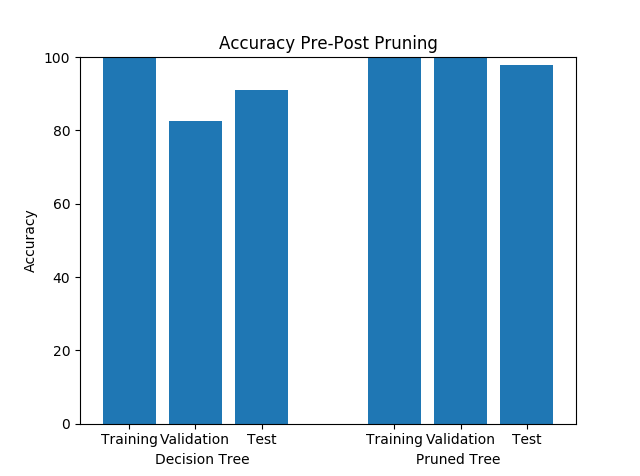
\includegraphics[width=\linewidth]{graph_breast_cancer_dataset.png}
	\caption{Grafico delle accuratezze in percentuale dell'albero prima e dopo la potatura}
	\label{imgGrafico}
\end{figure}


\section*{Conclusione}
Come previsto con l'operazione di potatura l'albero ha effettivamente avuto un overfitting minore rispetto a quello originale. L'accuratezza dell'albero sul Test Set si è avvicinata a quella sul Training set, portando il nostro albero a generalizzare correttamente nella quasi totalità dei casi.


\begin{thebibliography}{9}
\bibitem{norvig:relazione}
Norvig, Peter (2010),
\emph{Artificial Intelligence: A Modern Approach}, Pearson, New Jersey.
\bibitem{mitchell:relazione}
Tom M. Mitchell(1997),
\emph{Machine Learning}, McGraw-Hill.
\bibitem{site:relazione}
URL: https://en.wikipedia.org/wiki/Decision\_tree\_learning
\end{thebibliography}



\end{document}
